\documentclass[a4paper, 12pt]{article}

\usepackage[portuges]{babel}
\usepackage[utf8]{inputenc}
\usepackage{amsmath}
\usepackage{indentfirst}
\usepackage{graphicx}
\usepackage{multicol,lipsum}
\usepackage{cite}
\usepackage{hyperref}
\usepackage{float}
\usepackage{float}
\floatstyle{plaintop}
\restylefloat{table}
\usepackage{listings}





\begin{document}
%\maketitle

\begin{titlepage}
	\begin{center}

	%\begin{figure}[!ht]
	%\centering
	%\includegraphics[width=2cm]{c:/ufba.jpg}
	%\end{figure}

		\Huge{Universidade Federal de São Paulo}\\
		\large{Instituto de Ciência e Tecnologia}\\
		\large{Projetos em Engenharia da Computação}\\
		\vspace{15pt}
        \vspace{95pt}
        \textbf{\LARGE{Documentação do Site}}\\
		%\title{{\large{Título}}}
		\vspace{3,5cm}
	\end{center}

	\begin{flushleft}
		\begin{tabbing}
			Aluno: Davi Melo Morales\\
            Revisor: Gustavo Oliveira\\
            Professor: Dr. Arlindo Conceição
	\end{tabbing}
 \end{flushleft}
	\vspace{1cm}

	\begin{center}
		\vspace{\fill}
			 Junho\\
		 2016
			\end{center}
\end{titlepage}

\tableofcontents

\newpage

% % % % % % % % % % % % % % % % % % % % % % % % % % %



\section{Briefing}
\label{sec:briefing}

O desenvolvimento desse site diz respeito ao projeto \textit{Tomas - A Tomada Inteligente}, realizado dentro da disciplina de \textit{Projetos em Engenharia da Computação}, tendo sido desenvolvido para trabalhar em conjunto com outros componentes do projeto e auxiliar na comunicação com o cliente.

\subsection{Objetivos}

O site apresenta uma série de objetivos distintos, que são:

\begin{itemize}
\item Apresentar o produto ao cliente, informando seus recursos e especificações;
\item Proporcionar a aquisição do produto através de uma loja virtual;
\item Oferecer ao usuário a possibilidade de criar uma conta para uso do produto, assim como obter informações dele e controlá-lo remotamente;
\item Fornecer ao cliente informações quanto a dúvidas frequentes e proporcionar a comunicação direta da companhia com o cliente.
\end{itemize}

\subsection{Público Alvo}

\begin{itemize}
\item Pessoas interessadas em conhecer ou adquirir o produto;
\item Clientes que procuram monitorar e controlar seus produtos já adquiridos;
\item Pessoas que busquem por informações adicionais a respeito do produto, possuam dúvidas ou precisem de suporte.
\end{itemize}

\subsection{Ferramentas Utilizadas}

Toda a parte de \textit{front-end} foi elaborada sobre a \textit{framework Bootstrap}. As linguagens trabalhadas foram \textit{HTML}, \textit{CSS} e \textit{JavaScript}.

O controle de ações e comunicação com o servidor se realizaram com \textit{JavaScript} - pouco aplicado - e PHP associado a SQL, de maneira que as informações apresentadas no \textit{front-end} são recuperadas via SQL e dispostas através do PHP.

As ações e informações enviadas ao servidor via SQL são fornecidas sobre elementos do \textit{front-end} e organizadas ou tratadas através do PHP.

Os gráficos exibidos são gerados pela API \textit{Google Charts}, que funciona em \textit{JavaScript} associado ao \textit{PHP}, que fornece os dados para o script.

O nome de domínio foi obtido pelo serviço \textit{NOIP}, enquanto o carrinho de compras foi integrado através do serviço \textit{MOIP}.

O versionamento do \textit{site} foi realizado via \textit{git}, sendo que o projeto se encontra na íntegra no seguinte endereço do \textit{github}: "https://github.com/davimmorales/smartPlug-webpage".

\subsection{Informações Sobre a Equipe}

O projeto dessa etapa foi realizado pelo departamento de desenvolvimento do \textit{site}, o qual faz parte da divisão de \textit{Comunicação e Plataforma de Gerenciamento} da equipe de criação do \textit{Tomas}. Essa equipe é formada pelos alunos Davi Melo Morales e Gustavo Oliveira de Souza; houveram, também, contribuições da parte do José Henrique Fortes Leite.

O projeto apresenta uma identidade visual unificada, onde todos os produtos relacionados ao projeto se apresentam com as cores vermelho e preto - ou grafite. A Figura \ref{fig:logo} apresenta a logomarca utilizada.

\begin{figure}[!ht]
	\centering
	\resizebox{9cm}{!}{
	\includegraphics{Figures/logo.png}}
	\caption{Logotipo da marca}
	\label{fig:logo}
\end{figure}

\section{Arquitetura da Informação e Elementos de \textit{Layout}}

\subsection{\textit{Navbar}}

Esse elemento é presente em todas as páginas do \textit{site}. Ele organiza o acesso às categorias de base do \textit{site} de acordo com a tarefa que se deseja realizar ou com as informações procuradas. Apresenta-se de forma extensa sua forma padrão e em um \textit{menu sanduíche} em sua forma responsiva, conforme a Figura \ref{fig:navbar}. A seguir estão listadas as categorias presentes na \textit{navbar}:

\begin{itemize}
\item \textit{Home}: página inicial onde há informações a respeito do produto - apresentação de recursos;
\item Loja: ambiente destinado a quem deseja adquirir o produto;
\item Minha conta: seção apropriada a quem deseja acessar informações sobre ou controlar seus produtos adquiridos;
\item Suporte: área onde se pode obter ajuda e sanar dúvidas.
\end{itemize}

\begin{figure}[!ht]
	\centering
	\resizebox{13cm}{!}{
	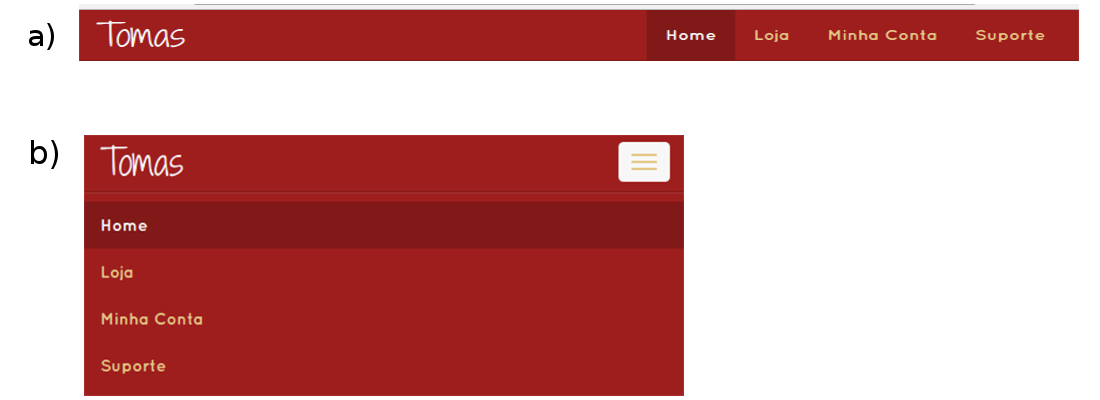
\includegraphics{Figures/navbar.png}}
	\caption{a: \textit{Navbar} em sua forma padrão;  b: \textit{Navbar} em sua forma responsiva.}
	\label{fig:navbar}
\end{figure}

O acesso às páginas se dá através do clique simples do \textit{mouse} em qualquer dessas categorias, sendo o acesso à \textit{Home} possível tanto através de seu título quanto através do título do produto presente no mesmo elemento.

\subsection{\textit{Home}}

A página \textit{Home} apresenta o produto, seus recursos e serviços de maneira gradual e explicativa, fazendo uso de imagens e vídeos explicativos. Os tópicos abordados nela são:

\begin{itemize}
\item A proposta do produto;
\item O recurso de controle remoto;
\item A possibilidade de programação das tomadas;
\item Demonstração das ferramentas de monitoramento dos dispositivos, mencionando benefícios econômicos dessa prática;
\item Menção ao suporte ao produto e sua possibilidade de extensão.
\end{itemize}

\subsection{Loja}

A Loja apresenta os produtos e serviços oferecidos ao cliente, sendo eles a \textit{base}, a \textit{tomada} e o \textit{suporte premium}. Abaixo de cada produto há um botão que adiciona uma unidade dele ao carrinho de compras.

A adição de um item ao carrinho de compras ou o clique em seu identificador - Figura \ref{fig:carrinho} - encaminham o usuário à página do carrinho de compras.

\begin{figure}[!ht]
	\centering
	\resizebox{5cm}{!}{
	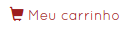
\includegraphics{Figures/carrinho.png}}
	\caption{Ícone do carrinho de compras.}
	\label{fig:carrinho}
\end{figure}

\subsubsection{Carrinho de Compras}

A página do carrinho de compras permite o controle quanto aos produtos adquiridos e sua quantidade. Eles são dispostos em uma tabela, a se organiza nas colunas: \textit{produto} - que identifica o produto por tipo -, \textit{quantidade}, \textit{remover} e \textit{valor unitário}.

Os itens \textit{remover} e \textit{quantidade} podem ser alterados pelo usuário.

Abaixo, há uma descrição do valor total da compra e os seguintes botões: \textit{continuar comprando} - o qual leva o usuário de volta à página da loja -, \textit{atualizar carrinho} - atualiza as alterações realizadas - e \textit{finalizar compra}, que leva o usuário a consumar sua aquisição e realizar o pagamento.

A Figura \ref{fig:carrinhopagina} apresenta um exemplo de configuração dessa página.

\begin{figure}[!ht]
	\centering
	\resizebox{13cm}{!}{
	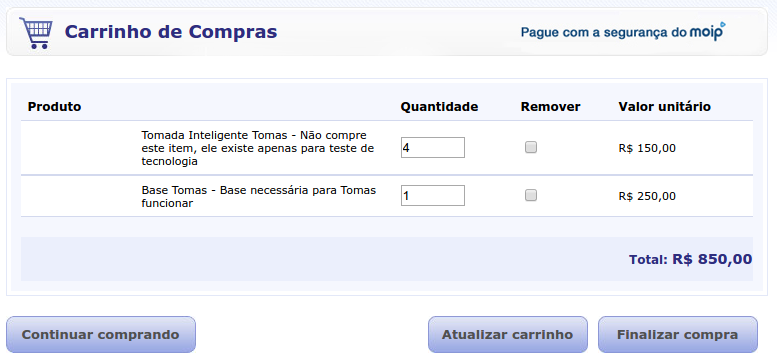
\includegraphics{Figures/carringopagina.png}}
	\caption{Página do carrinho de compras.}
	\label{fig:carrinhopagina}
\end{figure}

\subsection{Minha Conta}

A seção \textit{Minha Conta} se apresenta de duas formas: \textit{acesso} e \textit{controle}.

\subsubsection{Acesso}

Essa página apresenta dois formulários: o de \textit{login} e o de \textit{cadastro}.

Caso o usuário já possua cadastro no serviço, ele deverá fornecer seu \textit{e-mail} e senha cadastrados e clicar em "acesse sua conta" para ser encaminhado à página de controle.

Caso queira se cadastrar, o usuário deverá fornecer seu nome, e-mail, senha e repetir a digitação da senha. Ao clicar em \textit{crie sua conta}, caso a criação da conta seja realizada com sucesso, o usuário será encaminhado para sua página de controle.

\subsubsection{Falhas no Acesso}

O controle de acesso à página de controle é feito através de verificações no banco de dados do serviço por questões de segurança, organização e operabilidade.

Diante à tentativa de acesso à conta, é verificado se: todos os campos do formulário estão preenchidos, a validade do endereço de \textit{e-mail} e sua correspondência com a senha fornecida.

Quando se tenta criar uma conta, é verificado se: todos os campos do formulário estão preenchidos, o \textit{e-mail} já está cadastrado e se a \textit{senha} e sua verificação se correspondem.

Caso haja falha em qualquer dessas verificações, um \textit{modal} específico ao problema informa ao usuário o ocorrido e a página é atualizada. A Figura \ref{fig:modalErro} exemplifica um \textit{modal} de notificação de erro.

\begin{figure}[!ht]
	\centering
	\resizebox{13cm}{!}{
	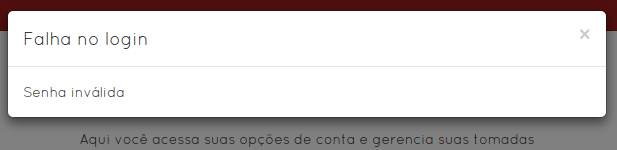
\includegraphics{Figures/erroModal.png}}
	\caption{Exemplo de notificação de erro no \textit{login}.}
	\label{fig:modalErro}
\end{figure}

\subsubsection{Controle e Monitoramento}

Feito o acesso à conta, o usuário é encaminhado para essa página, a qual o permite cadastrar, remover, controlar, programar e monitorar seus dispositivos adquiridos.

A página conta com uma barra superior de boas vindas, logo abaixo da \textit{navbar}, que o saúda pelo nome cadastrado e lhe permite fazer o \textit{logout}.

Dispõem-se, então, as tomadas cadastradas em uma tabela à esquerda da tela, enquanto os gráficos de monitoramento se localizam à direita, conforme a Figura \ref{fig:controle}. Essa tabela apresenta os seguintes campos: \textit{número}, \textit{nome} e \textit{estado}, sendo que este pode ser alterado através do clique no campo que lhe descreve.

\begin{figure}[!ht]
	\centering
	\resizebox{13cm}{!}{
	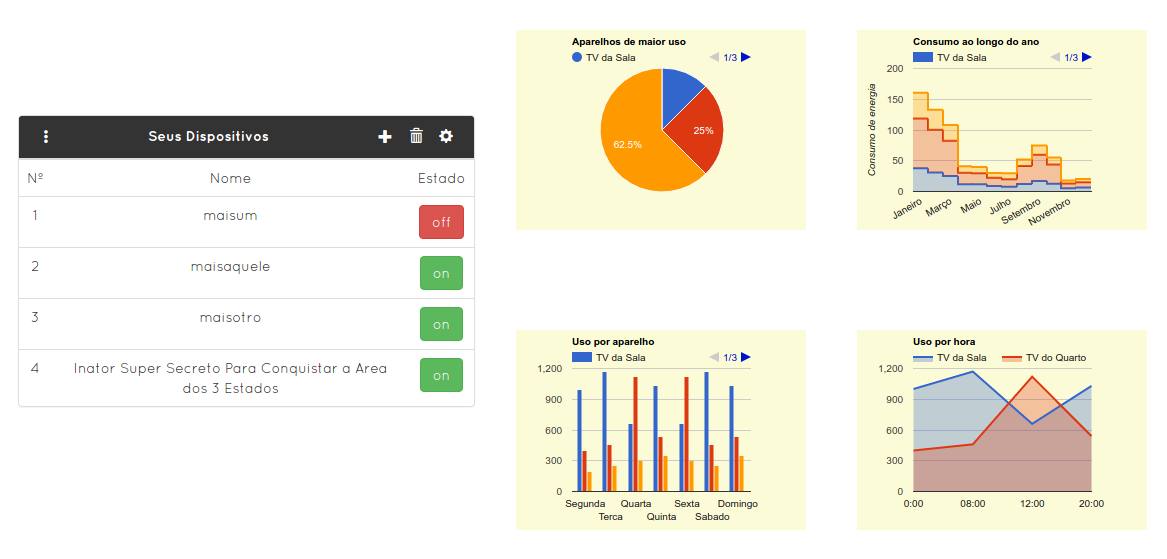
\includegraphics{Figures/controle.png}}
	\caption{Exemplo de disposição da página de controle e monitoramento.}
	\label{fig:controle}
\end{figure}

Sobre a tabela de dispositivos, há uma barra de tarefas que apresenta os seguintes signos: \textit{3 pontos}, \textit{mais}, \textit{lixeira} e \textit{engrenagem}. Eles são botões e proporcionam o acesso a funções distintas:

\begin{itemize}
\item 3 pontos: permite a alteração de nome do dispositivo cadastrado;
\item Mais: fornece a opção de adicionar uma tomada, informando-se os campos: \textit{nome} e \textit{número de série};
\item Lixeira: apresenta a opção de exclusão de dispositivo, Figura \ref{fig:lixeira};
\item Engrenagem: traz as opções de programação da tomada - com o estado desejado, dia e horário para a criação do evento -, assim como uma lista dos eventos programados e a opção de removê-los, conforme a Figura \ref{fig:modalControle}.
\end{itemize}

\begin{figure}[!ht]
	\centering
	\resizebox{9cm}{!}{
	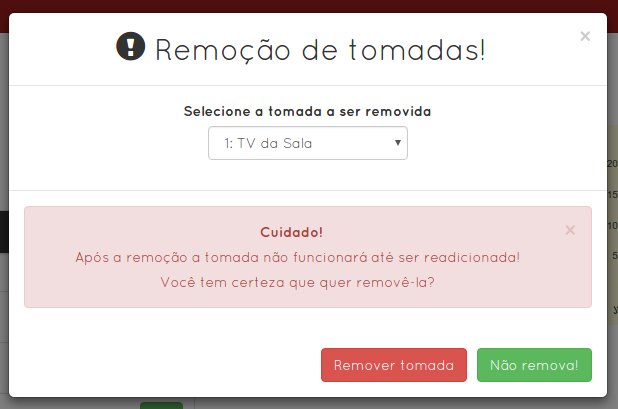
\includegraphics{Figures/lixeira.png}}
	\caption{Modal referente ao \textit{menu} de exclusão de dispositivos.}
	\label{fig:lixeira}
\end{figure}

\begin{figure}[!ht]
	\centering
	\resizebox{13cm}{!}{
	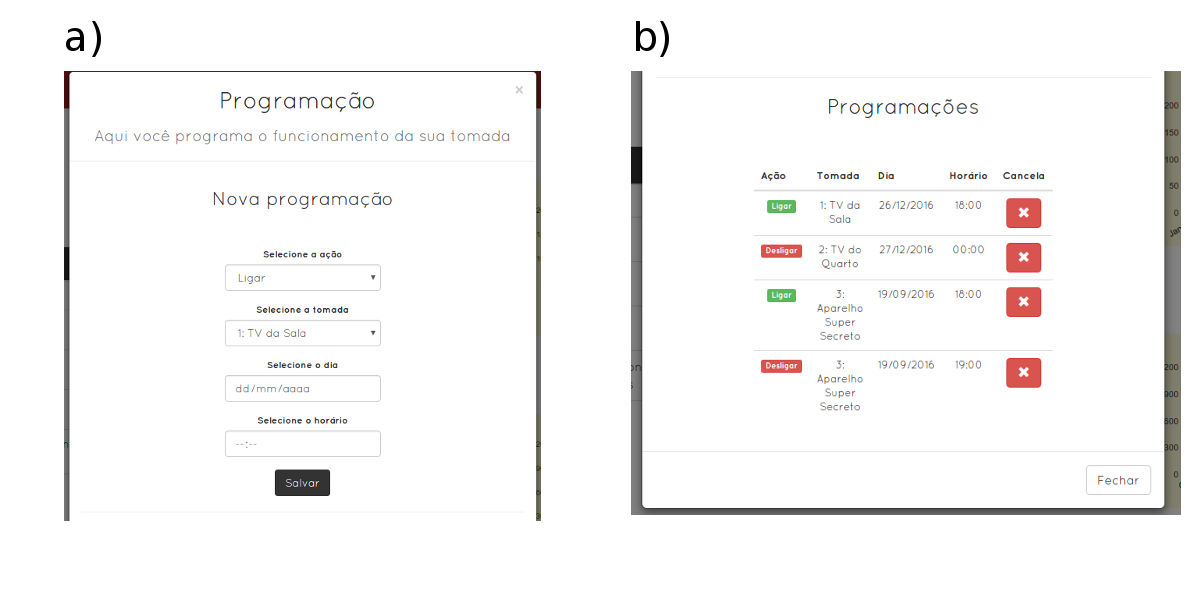
\includegraphics{Figures/modalControle.png}}
	\caption{Modal referente à programação dos dispositivos: a) \textit{menu} de criação de eventos; b) disposição dos eventos já criados. }
	\label{fig:modalControle}
\end{figure}

\subsection{Suporte}

A página de suporte apresenta um formulário com os campos \textit{nome}, \textit{endereço de e-mail} e \textit{mensagem} - conforme a Figura \ref{fig:suporte}, a fim de que o usuário possa se comunicar com a equipe de atendimento para sanar dúvidas e informar problemas.

\begin{figure}[!ht]
	\centering
	\resizebox{13cm}{!}{
	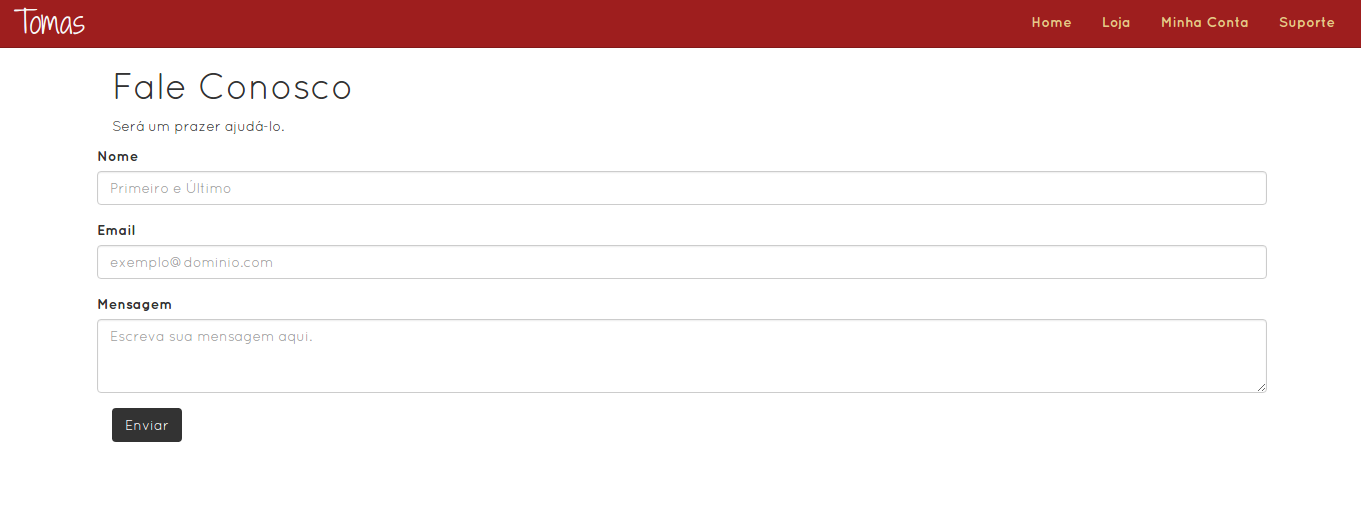
\includegraphics{Figures/suporte.png}}
	\caption{Página de atendimento ao cliente.}
	\label{fig:suporte}
\end{figure}

\end{document}
